\section{Wind instruments}
\bi

\i We continue in this section with our discussion 
of musical instruments.

\i Here we will focus on three wind instruments:
a flue-organ pipe, a penny whistle, and a clarinet.
(We will briefly describe brass instruments at the end 
of the section.)

\i As before, we will follow the presentation of ``How music works,"
by John Powell.

\ei
%%%%%%%%%%%%%%%%%%%%%%%%%%%%%%%%%%%%%%%%%%%%%%
\subsection{Sounds from wind in tubes}
\bi

\i Wind instruments come in two basics types:
those that have reeds and those that don't.

\i Examples of wind instruments that have reeds 
are the clarinet, oboe, bassoon, ...
(Oboes and bassoons actually have double reeds.)
Examples of wind instruments that don't have reeds
are the flue-organ pipe, penny whistle, flute, recorder, ...

\i For both types of wind instruments, the
sound is produced by a vibrating air column 
in a tube.

\i The vibrations in the air column are 
excited by either an
{\em oscillating air stream} directed over an
edge (like that from a whistle) or a 
{\em vibrating reed}.
(For brass wind instruments, a vibrating reed
is replaced by the vibrating lips of a brass player.)

\i We will discuss these different sources of
excitation in the next two subsections.

\i For both types of excitation, the oscillation 
frequency of the air stream or the vibration
frequency of the reed (or lips) 
is determined (via resonance) by
the natural frequencies of the air column in the tube.  

\i Recall that the natural frequencies of an
air column in a tube depend on two things, 
in addition to the speed of sound in air:
(i) the length of the tube, and 
(ii) whether the tube 
is closed at one or open at both ends.

\i Mathematically, the frequency of the nth 
standing wave vibration of an air column
in a cylindrical tube is given by:

Tube open at both ends:
%
\be
f_n = n\left(\frac{v}{2L}\right)\,,
\qquad
n=1,2,3,\cdots
\label{e:open}
\ee
%
Tube open at one end, closed at the other:
%
\be
f_n = n\left(\frac{v}{4L}\right)\,,
\qquad
n=1,3,5,\cdots
\label{e:closed}
\ee
%
where $L$ is the length of the tube and 
$v$ is the speed of sound in air 
($v=346~{\rm m/s}$ at room temperature).

\i We are assuming that the tubes are sufficiently
narrow so that end effects are not important.
Otherwise, we would have to increase the effective 
length of the tube by $0.61 R$ for each open end,
where $R$ is the radius of the tube.

\i Note that for tubes closed at one end,
only odd harmonics are present.
Tubes open at both ends have both even and odd 
harmonics.

\ei
%%%%%%%%%%%%%%%%%%%%%%%%%%%%%%%%%%%%%%%%%%%%%%
\subsection{Oscillating air streams}
\bi

\i An oscillating air stream is an example of 
a {\em flow-controlled} excitation, associated 
with the displacement of the air molecules.

\i Figure~\ref{f:edge} shows what happens 
to a stream of air as it encounters a sharp
edge.
%
\begin{figure}[htbp]
\begin{center}
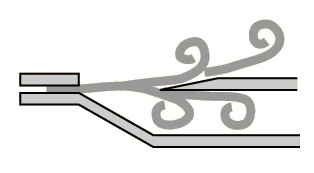
\includegraphics[width=.5\textwidth]{edge.jpg}
\caption{Schematic diagram showing an air 
stream encountering a sharp edge.
The stream splits into vortices that take 
turns going to one side or the other of the edge.
(Figure taken from 
{\tt hyperphysics.phy-astr.gsu.edu/}.)}
\label{f:edge}
\end{center}
\end{figure}

\i Note that the air stream doesn't divide 
into two smoothly flowing streams on each 
side of the edge.
Instead, whirlpools (or vortices) are created,
which take turns going to one side or the 
other of the edge.
(This is analogous to cars in traffic deciding
to go to either one side or the other of 
a divider in the road, based on the choice of
the previous cars.)

\i The frequency with which the vortices
are formed on opposite sides of the edge
is determined by the natural frequencies of 
the tube to the right of the edge.
Resonance occurs when the frequency of 
vortex formation matches one of the natural 
frequencies of the air column in the tube.

\i At resonance, a vortex enters the tube 
when the motion of the air molecules in the air 
column is also directed into the tube.

\i Since the vortices are associated with
air molecule motion, the location of the 
sharp edge is an {\em anti-node} for air molecule 
displacement (or a node for pressure deviation), 
and thus corresponds to an {\em open} end of a tube.
If the other end of the tube is open, 
then Equation~\ref{e:open} 
should be used for the natural frequencies.
If the other end of the tube is closed, 
then Equation~\ref{e:closed} should be used.

\i This is the basic operation of a 
whistle, or producing a sound by blowing
over a bottle.

\i \ex For a bottle-shaped object like that in 
Figure~\ref{f:helmholtzresonator},
called a {\em Helmholtz resonator},
there is only one natural frequency given by
%
\be
f = \frac{v}{2\pi}\sqrt{\frac{A}{Vl}}
\ee
%
where $l$ is the length of the neck, $A$ is its
cross-sectional area, $V$ is the volume of 
the base, and $v$ is the speed of sound in air.
%
\begin{figure}[htbp]
\begin{center}
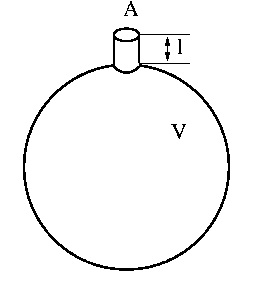
\includegraphics[width=.3\textwidth]{helmholtzresonator.jpg}
\caption{Schematic diagram of a bottle-shaped object, 
called a Helmholtz resonator.
(Figure taken from {\tt http://fisicaondemusica.unimore.it}.)}
\label{f:helmholtzresonator}
\end{center}
\end{figure}

\i The air in the neck acts like a mass 
$m = \rho A l$ attached to a spring with spring constant
$K = {\rho A^2 v^2}/{V}$, where $\rho$ is the density
of the air.

\i The body of a guitar or violin with its sound hole acts
like a Helmholtz resonator.

\i \demo
Calculate the resonant frequency of a bottle,
approximating the neck length, cross-sectional area of the
neck, and volume of the base.
Blow over the lip of the bottle to produce a sound, and
use iSpectrum to determine its fundamental frequency.
How well does the calculated frequency agree 
with measured frequency?

\ei
%%%%%%%%%%%%%%%%%%%%%%%%%%%%%%%%%%%%%%%%%%%%%%
\subsection{Vibrating reeds and tubes}
\bi

\i A vibrating reed (or vibrating lips) is an 
example of a {\em pressure-controlled} excitation,
associated with pulses of high and low pressure 
waves.

\i Figure~\ref{f:pipe-reed-system} shows what
happens to a pressure pulse as it propagates in
an open tube with a reed at one end.
%
\begin{figure}[htbp]
\begin{center}
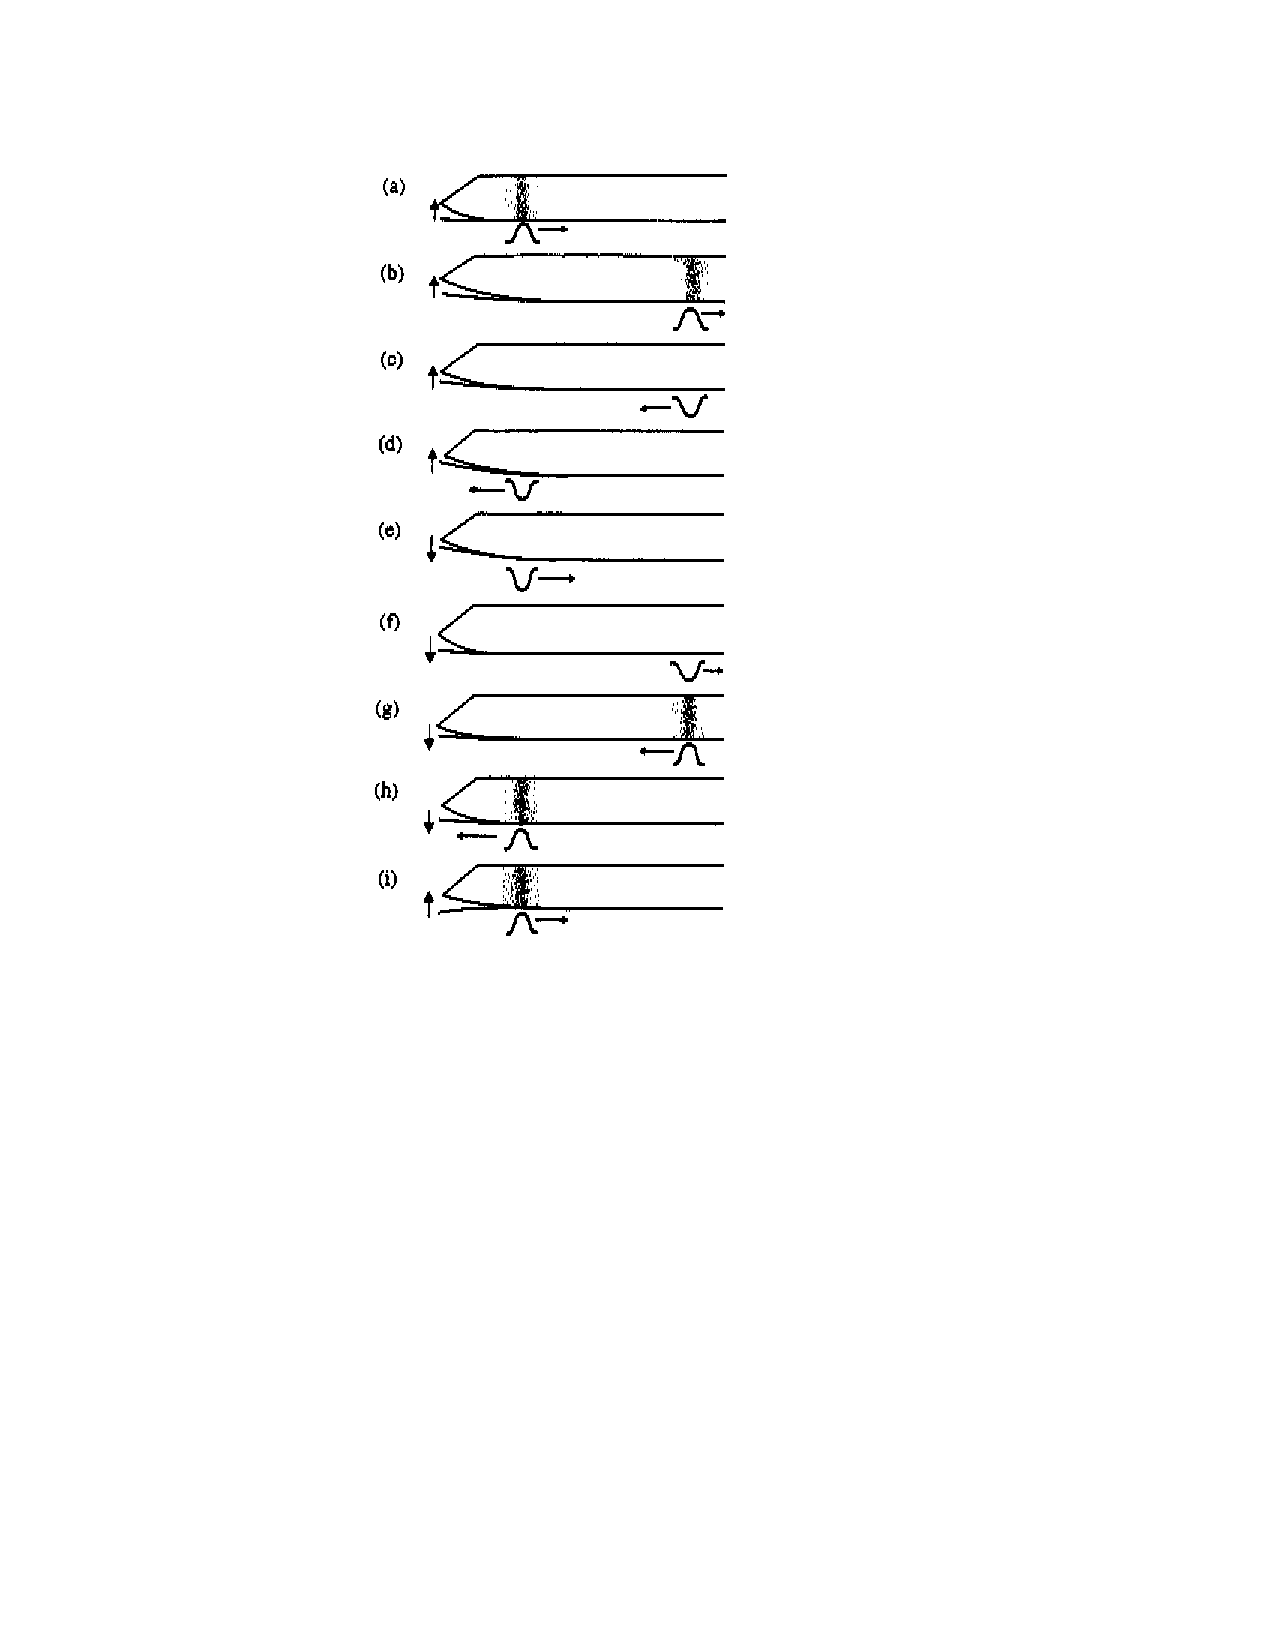
\includegraphics[height=.9\textheight]{pipe-reed-system.pdf}
\caption{Schematic diagram showing 
positive and negative-pressure pulses 
propagating in
an open tube with a reed at one end.
(Figure taken from ``Science of Sound,"
by Rossing, Moore, and Wheeler.)}
\label{f:pipe-reed-system}
\end{center}
\end{figure}

(a)-(b): When the reed is open, a positive-pressure
pulse enters the tube and propagates to the right.

(c): At the open end of the tube, the 
positive-pressure pulse is inverted upon reflection, 
becoming a negative-pressure pulse.
(Recall that an open end of a tube is a node 
for pressure deviations, or an anti-node for air 
molecule displacement.)

(d): The negative-pressure pulse then propagates 
to the left, reaching the reed-end of the tube, helping
to draw the reed shut.
No air enters the tube at this time.

(e): The negative-pressure pulse sees the 
reed-end of the tube as a closed end, and hence 
is {\em not} inverted upon reflection.

(f)-(g): The negative-pressure pulse propagates 
to the right and reflects off the open end of the tube.

(h)-(i): The returning positive-pressure pulse 
now helps to keep the reed open,
allowing an external high-pressure pulse of air
to enter the tube.

The whole process repeats as in (a).

\i \underline{Summary}: 
At resonance, the reed acts like a pressure-controlled valve, 
letting in high-pressure pulses of air in phase
with the high-pressure vibrations of the air column in the tube.

\i Note that the reed is closed for half a cycle,
during which time no energy is added to the air column
in the tube.
This is similar to the slipping stage of a bowed violin string.

\i Since a reed acts like a closed end of a tube,
the natural frequencies of the vibrating air column 
consist of only the {\em odd} harmonics.

\ei
%%%%%%%%%%%%%%%%%%%%%%%%%%%%%%%%%%%%%%%%%%%%%%
\subsection{Flue-organ pipe}
\bi

\i A flue-organ pipe is an example of a wind
instrument that uses an oscillating air stream as
its source of excitation.

\i When an organ key is pressed, a 
constant flow of air is directed toward a 
sharp edge at one end of the organ pipe,
as shown in Figure~\ref{f:fluepipe}.
%
\begin{figure}[htbp]
\begin{center}
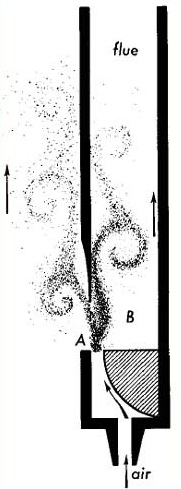
\includegraphics[width=.3\textwidth]{fluepipe.jpg}
\caption{Schematic diagram showing air flow
in a flue-organ pipe.
(Figure taken from {\tt http://home.comcast.net}.)}
\label{f:fluepipe}
\end{center}
\end{figure}

\i Since the oscillating air stream acts like
an open end of a tube, the natural frequencies
of the vibrating air column depend on whether
the other end of the flue-organ pipe is open or closed.

\i If the other end of the pipe is closed, then 
only odd harmonics are produced.

\i There are also reed-organ pipes, where
the sharp edge of the pipe is basically replaced 
by a vibrating reed.
(See pipes 4 and 5 in Figure~\ref{f:pipes}.)
%
\begin{figure}[htbp]
\begin{center}
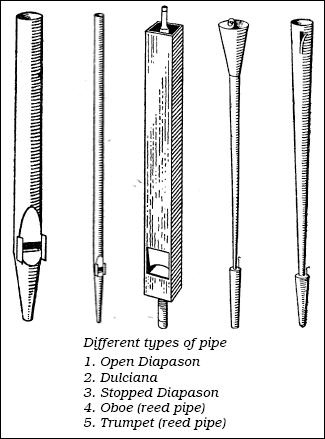
\includegraphics[height=.5\textwidth]{pipes.png}
\caption{Different types of organ pipes.
Flue-organ pipes (1-3) and reed-organ pipes (4, 5).
(Figure taken from 
{\tt http://www.churchmusicdublin.org/}.)}
\label{f:pipes}
\end{center}
\end{figure}

\i The timbre of a note produced by an organ pipe is 
affected by the shape of the bore (e.g., whether 
it is cylindrical or conical), whether it is open 
or closed at the other end, and how wide it is.
Narrow pipes support higher harmonics better than 
wide pipes.

\i But like a harp, each organ pipe basically 
produces only one note.
To get more than one note per pipe, you need 
to drill holes in it, like a penny whistle, which
we describe next.

\ei
%%%%%%%%%%%%%%%%%%%%%%%%%%%%%%%%%%%%%%%%%%%%%%%%
\subsection{Penny whistle}
\bi

\i A penny whistle is like an organ pipe, but with 
a series of holes drilled in it.
%
\begin{figure}[htbp]
\begin{center}
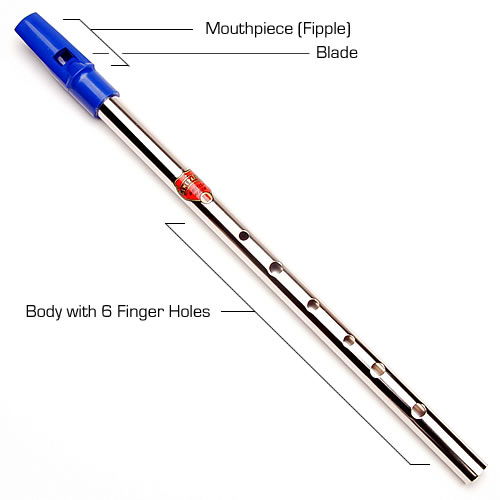
\includegraphics[height=.5\textwidth]{pennywhistle.jpg}
\caption{A penny whistle.
{\tt http://www.blaynechastain.com/files/webfm/image/course-whistle/}.)}
\label{f:pennywhistle}
\end{center}
\end{figure}

\i These holes are called {\em tone holes}.
They allow you to play different notes, by selectively covering
or uncovering one or more holes with your fingers.

\i With all the tone holes covered, the effective length of
the tube is just the full length of the tube.

\i By uncovering a tone hole, you change the effective length
of the tube as shown in Figure~\ref{f:tonehole}.
Note that effective length depends on the 
{\em size} of the tone hole.
If the radius of the tone hole is the same as the radius of 
the tube, then the effective length of the tube ends at the
center of the tone hole.
%
\begin{figure}[htbp]
\begin{center}
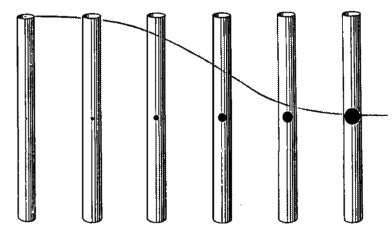
\includegraphics[height=.5\textwidth]{tonehole.jpg}
\caption{How the effective length of a tube depends
on the size of an open tone hole.
(Figure taken from {\tt http://www.physics.georgetown.edu/}.)}
\label{f:tonehole}
\end{center}
\end{figure}

\i There are 6 tone holes on a penny whistle corresponding 
to the 7 different notes of a diatonic scale.

\i By {\em partially} covering a tone hole with your finger, 
you get notes {\em in between} those defined by the fully-open 
(or fully-closed) tone holes.

\i By {\em overblowing} a penny whistle (i.e., blowing with 
more force than normal), one can excite the second
(or even third) harmonic  
of the vibrating air column, and hence produce notes that are
an octave (or a twelfth) above the nominal notes.

\ei
%%%%%%%%%%%%%%%%%%%%%%%%%%%%%%%%%%%%%%%%%%%%%%
\subsection{Clarinet}
\bi

\i A clarinet is an example of a reed-pipe system.

\i Figure~\ref{f:clarinet} shows the parts of a clarinet
and Figure~\ref{f:reed-schematic} is a schematic
drawing of the reed.
%
\begin{figure}[htbp]
\begin{center}
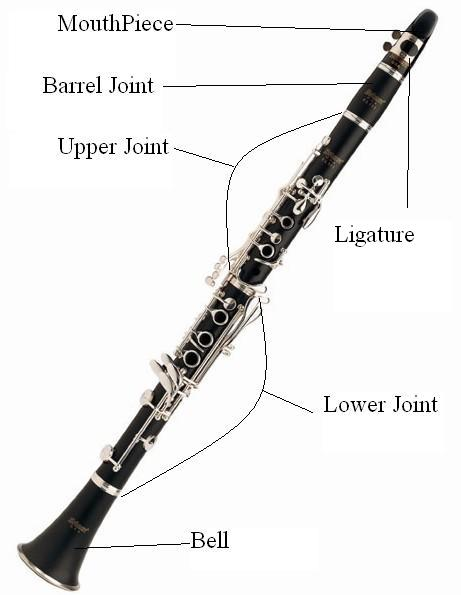
\includegraphics[height=.5\textheight]{clarinet.jpg}
\caption{Parts of a clarinet.
(Figure taken from {\tt http://en.wikibooks.org/wiki/Clarinet}.)}
\label{f:clarinet}
\end{center}
\end{figure}
%
\begin{figure}[htbp]
\begin{center}
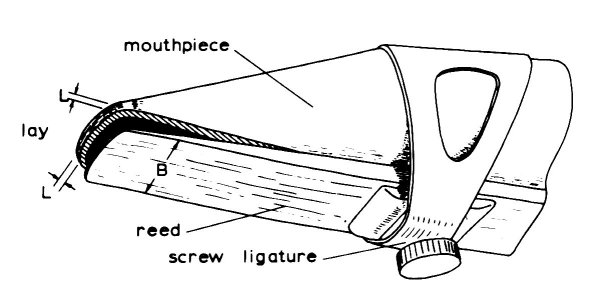
\includegraphics[width=.4\textwidth]{reed-schematic.jpg}
\caption{Schematic diagram of a clarinet reed.
(Figure taken from 
{\tt http://www.speech.kth.se/music/publications/leofuks/thesis/}.)}
\label{f:reed-schematic}
\end{center}
\end{figure}

\i The vibration frequency of the reed is determined
by resonance to match the natural frequencies
of vibration of the air column in the tube.
(These vibration frequencies are typically much less than 
the natural frequency of the reed by itself.)

\i Since a clarinet has a cylindrical bore and is closed
at one end (because of the reed), {\em odd} harmonics are
predominantly produced.
(The conical shape of the bell changes the higher harmonics 
slightly.)

\i NOTE:
For reed instruments with conical bores, {\em both} even 
and odd harmonics are produced.

\i Because the reed acts as a closed end for a clarinet,
its fundamental frequency is an octave lower than that of 
a flute, even though they both have the same size.
(This is because a flute acts like a tube that is open at 
{\em both} ends.)

\i Similarly, because of the reed, overblowing a clarinet 
will produce notes that are a twelfth (three times) above 
the nominal notes.

\i In addition to tone holes, clarinets have 
{\em register keys} that allow you to
play notes in a higher register (pitch) than normal.

\i By opening the register key located a third of the way
from the reed-end of the clarinet, you produce a note
that is a musical twelfth 
(or {\em three} times the fundamental) 
higher than with the register key closed, as shown in
Figure~\ref{f:registerkey}.
(One gets the third harmonic, and not the second, since a 
clarinet produces only the odd harmonics.)
%
\begin{figure}[htbp]
\begin{center}
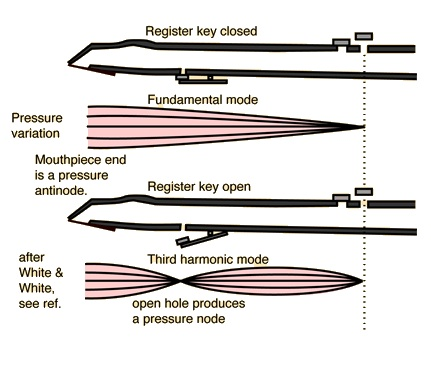
\includegraphics[width=.9\textwidth]{registerkey.jpg}
\caption{The operation of a clarinet register key.
The vertical dotted line shows the location of an open
tone hole, which defines the effective length of the
clarinet tube.
(Figure taken from 
{\tt http://hyperphysics.phy-astr.gsu.edu}.)}
\label{f:registerkey}
\end{center}
\end{figure}

\ei
%%%%%%%%%%%%%%%%%%%%%%%%%%%%%%%%%%%%%%%%%%%%%%
\subsection{Brass instruments (in brief)}
\bi

\i Brass instruments are similar to woodwind instruments in 
that the vibrating lips of a brass player play the same role as
a vibrating reed in e.g., a clarinet.

\i But since a brass player's lips are {\em more massive} 
than a reed on a woodwind instrument, the brass player
can more easily play harmonics on his (or her) instrument
by simply buzzing his lips at the harmonic frequencies of
the vibrating air column in the tube.
(No valves or slides are needed to play these harmonic notes.)

\i Brass instruments differ from woodwind instruments in that 
they use valves (for trumpets and tubas) and slides 
(for trombones) to change the effective length of the air column, 
instead of using tone holes and register keys.

\i Since there are no tone holes for brass instruments, 
most of the sound is radiated from the {\em bell} of the instrument.

\i Since a trumpet has a cylindrical bore and the lips act like
a closed end of a tube, one might think that a trumpet should produce 
only odd harmonics.
But the mouthpiece and the bell change the natural frequencies
of the instrument, so that both even and odd harmonics are actually
produced.

\ei
